% !TEX program = pdflatex
% !TEX options = -synctex=1 -interaction=nonstopmode -file-line-error "%DOC%"
% 作业模板
\documentclass[UTF8,10pt,a4paper]{article}
\usepackage{ctex}
\newfontfamily\menlo{MONACO.TTF}
\usepackage{amsmath}
\usepackage{diagbox}
\usepackage{float}
\usepackage{listings}
\usepackage{multirow}
\usepackage{tabularx}

\usepackage{url}
\usepackage{xcolor}
\newcommand{\tabincell}[2]{\begin{tabular}{@{}#1@{}}#2\end{tabular}}

\lstset{
    breaklines,                                 % 自动将长的代码行换行排版
    extendedchars=false,                        % 解决代码跨页时,章节标题,页眉等汉字不显示的问题
    backgroundcolor=\color[rgb]{0.96,0.96,0.96},% 背景颜色
    keywordstyle=\color{blue}\bfseries,         % 关键字颜色
    identifierstyle=\color{black},              % 普通标识符颜色
    commentstyle=\color[rgb]{0,0.6,0},          % 注释颜色
    stringstyle=\color[rgb]{0.58,0,0.82},       % 字符串颜色
    showstringspaces=false,                     % 不显示字符串内的空格
    numbers=left,                               % 显示行号
    numberstyle=\tiny\menlo,                    % 设置数字字体
    basicstyle=\small\menlo,                    % 设置基本字体
    captionpos=t,                               % title在上方(在bottom即为b)
    frame=single,                               % 设置代码框形式
    rulecolor=\color[rgb]{0.8,0.8,0.8},         % 设置代码框颜色
}  

\usepackage{pythonhighlight}
\usepackage{listings}
\usepackage{xcolor}
\usepackage{graphicx}
\usepackage[a4paper,left=2cm,right=2cm,top=2cm,bottom=2cm]{geometry}
\usepackage{fancyhdr}
% \catcode`\。=\active
% \newcommand{。}{.}
\newcommand{\CourseName}{操作系统(Operating System)}
\newcommand{\CourseCode}{CS307 \& CS356}
\newcommand{\Semester}{2020-2021学年第二学期}
\newcommand{\ProjectName} {\Huge{Project 2}} 
\newcommand{\StudentName}{刘涵之}
\newcommand{\StudentID}{519021910102}
\usepackage[vmargin=1in,hmargin=.5in]{geometry}
\usepackage{fancyhdr}
\usepackage{lastpage}
\usepackage{calc}
\pagestyle{fancy}
\fancyhf{}
\fancyhead[L]{\CourseName}
\fancyhead[C]{\ProjectName}
\fancyhead[R]{\StudentName}
\fancyfoot[R]{\thepage\ / \pageref{LastPage}}
\setlength\headheight{12pt}
\fancypagestyle{FirstPageStyle}{
    \fancyhf{}
    \fancyhead[L]{\CourseName\\
        \CourseCode\\
        \Semester}
    \fancyhead[C]{\large\bfseries\ProjectName \\}
    \fancyhead[R]{Name: \makebox[\widthof{\StudentID}][s]{\StudentName}\\
        ID : \StudentID\\
        }
    \fancyfoot[R]{\thepage\ / \pageref{LastPage}}
    \setlength\headheight{36pt}
}
\usepackage{amsmath,amssymb,amsthm,bm}
\allowdisplaybreaks[4]
\newtheoremstyle{Problem}
{}
{}
{}
{}
{\bfseries}
{.}
{ }
{第\thmnumber{ #2}\thmname{ #1}\thmnote{ (#3)} 得分: \underline{\qquad\qquad}}
\theoremstyle{Problem}
\newtheorem{prob}{题}
\newtheoremstyle{Solution}
{}
{}
{}
{}
{\bfseries}
{:}
{ }
{\thmname{#1}}
\makeatletter
\def\@endtheorem{\qed\endtrivlist\@endpefalse}
\makeatother
\theoremstyle{Solution}
\newtheorem*{sol}{解}
\title{Project 2: UNIX Shell Programming \& Linux Kernel Module for Task Information}
\date{}
% \usepackage{graphicx}
\begin{document}
\maketitle
\thispagestyle{FirstPageStyle}


\section{UNIX Shell Programming}
In this task, i will implement a UNIX Shell with following parts:
\begin{itemize}
    \item[(1)] Creating the child process and executing the command in the child
    \item[(2)] Providing a history feature
    \item[(3)] Adding support of input and output redirection
    \item[(4)] Allowing the parent and child processes to communicate via a pipe
\end{itemize}

\textbf{Design:} My key designs is as follows:
\begin{itemize}
    \item To parse the input command, i use \textbf{flatten()} function to remove extra space, then i use \textbf{tokenize()} function to transform string into array.
    \item After parsing, i check whether it is \texttt{!!} or \texttt{exit}, and give the result.
    \item Then i use \textbf{fork()} function to create the child process. The instruction will be execute in the child process.
    \item Then i use \textbf{concurrentFlag} function to check whether it asks for concurrent execution. If true, the parent process will not execute \texttt{wait(NULL)}. If false, the parent process will wait until the child process is done.
    \item In the child process, then i check whether the instruction needs a pipe. If true, \textbf{pipe(pipe\_fd)} will be called to generate a pipe. It will be used to carry out data communication.
    \item If the instruction need to be redirected, \textbf{dup2()} function is used to redirect the input/output.
    \item As for the concrete instruction such as \textbf{ls}, i use \textbf{execvp()} to execute it.
    
\end{itemize}


The code of simple-shell.c is shown as follows.
\begin{lstlisting}[language = c]
#include <stdio.h>
#include <unistd.h>
#include <stdlib.h>
#include <string.h>
#include <sys/wait.h>
#include <fcntl.h>

#define MAX_LINE		80 /* 80 chars per line, per command */
#define bool			int /* simulate boolean... */
#define true			1
#define false			0

void flatten(char *a, char *b) { // remove extra space, \n, \t
	int length = strlen(a);
	int current_location = 0;
	bool blank_end = false;
	for (int i = 0; i < length; i++) {
		if (a[i] == ' ' || a[i] == '\t' || a[i] == '\n') {
			if (blank_end) {
				b[current_location++] = ' ';
			}
			blank_end = false;
		} else {
			b[current_location++] = a[i];
			blank_end = true;
		}
	}
	if (b[current_location - 1] == ' ') {
		b[current_location - 1] = 0;
	}
	return;
}

int tokenize(char *a, char **b) {  //tokenize flatten string
	int num = 0; // token num
	int current_location = 0; // location inside string
	int length = strlen(a);
	if (length == 0) return 0;
	for(int i = 0; i < length; i++) {
		if (a[i] == ' ') {
			num++;
			current_location = 0;
		} else {
			b[num][current_location++] = a[i];
		}
	}
	return num + 1;
}

bool concurrentFlag(char *a) {
	int length = strlen(a);
	if (length == 0) return false;
	return (a[length - 1] == '&');
}

int main(void) {
	char *args[MAX_LINE/2 + 1];	/* command line (of 80) has max of 40 arguments */
	char *raw_string;
	char *flatten_string;
	char *last_command;
    int should_run = 1;
	bool have_last_command = false;
	raw_string = (char*) malloc(MAX_LINE * sizeof(char));
	flatten_string = (char*) malloc(MAX_LINE * sizeof(char));
	last_command = (char*) malloc(MAX_LINE * sizeof(char));
    while (should_run){   
		if (concurrentFlag(flatten_string) == false) wait(NULL);
        printf("\033[42;37mosh>\033[2;7;0m"); // pretty print ~
        fflush(stdout);
		memset(raw_string, 0, sizeof(raw_string));
		memset(flatten_string, 0, sizeof(raw_string));
		fflush(stdout);
        fgets(raw_string, MAX_LINE, stdin);
		flatten(raw_string, flatten_string); // remove space \t \n from raw_string

		if (strcmp(flatten_string, "exit") == 0) {
			should_run = 0;
			break;
		}
		if (strcmp(flatten_string, "!!") == 0) {
			if (have_last_command) {
				strcpy(flatten_string, last_command);
				fprintf(stdout, "%s\n", flatten_string);
			} else {
				fprintf(stderr, "No commands in history.\n");
				continue;
			}
		} else {
			have_last_command = true;
			strcpy(last_command, flatten_string);
		}

		pid_t pid;
		pid = fork();
		if (pid < 0) {
			fprintf(stderr, "Failed when creating a child process.\n");
			continue;
		}
		if (pid == 0) { // child
			for (int i = 0; i < MAX_LINE/2 + 1; i++) {
				args[i] = (char*) malloc(MAX_LINE * sizeof(char));
				memset(args[i], 0, sizeof(args[i]));
			}
			int command_num = tokenize(flatten_string, args);
			for (int i = command_num; i < MAX_LINE/2 + 1; i++) {
				free(args[i]);
				args[i] = NULL; 
			}
			
			if (concurrentFlag(flatten_string)) {
				free(args[command_num - 1]);
				args[command_num - 1] = NULL;
				command_num = command_num - 1;
			}

			int pipe_loc = -1;
			for (int i = 0; i < command_num; i++) {
				if (strcmp(args[i], "|") == 0) {
					pipe_loc = i;
					break;
				}
			}

			if (pipe_loc != -1) { // if pipe is need
				if (pipe_loc == 0 || pipe_loc == command_num -1) {
					fprintf(stderr, "Pipe command can't be conducted, expect more commands.\n");
				} else {
					int pipe_fd[2];
					int pipe_flag = pipe(pipe_fd);
					if (pipe_flag == -1) {
						fprintf(stderr, "Pipe can't be established.\n");
					} else { // pipe is created and no error, just do it ~
						pid = fork();
						if (pid < 0) {
							fprintf(stderr, "Failed when creating a child process.\n");
						}
						if (pid == 0) { // child of child
							for (int i = pipe_loc; i < command_num; i++) {
								free(args[i]);
								args[i] = NULL;
							}

							close(pipe_fd[0]); // close read
							if (dup2(pipe_fd[1], STDOUT_FILENO) < 0) {
								fprintf(stderr, "Dup failed.\n");
							} else {
								execvp(args[0], args);
							}
							close(pipe_fd[1]); // close write

							for (int i = 0; i < pipe_loc; i++) { // child of child menmory free
								free(args[i]);
							}
							free(raw_string);
							free(flatten_string);
							free(last_command);
							exit(0);
						} else { // child
							wait(NULL);

							for (int i = 0; i <= pipe_loc; i++) {
								free(args[i]);
							}
							for (int i = pipe_loc + 1; i < command_num; i++) { // move 2nd command to 1st
								args[i - pipe_loc - 1] = args[i];
							}
							for (int i = command_num - pipe_loc - 1; i < command_num; i++) {
								args[i] = NULL;
							}
							command_num = command_num - pipe_loc - 1;

							close(pipe_fd[1]);
							if (dup2(pipe_fd[0], STDIN_FILENO) < 0) {
								fprintf(stderr, "Pipe dup failed.\n");
							} else {
								execvp(args[0], args);
							}
							close(pipe_fd[0]);
						}
					}
				}
			} else { // no pipe, consider redirect input/output
				bool input_redirect_flag = false;
				bool output_redirect_flag = false;
				char *file_name;
				file_name = (char*) malloc(MAX_LINE * sizeof(char));
				if (command_num >= 3) {
					if ((strcmp(args[command_num - 2], "<") == 0) || (strcmp(args[command_num - 2], ">") == 0)) {
						if (strcmp(args[command_num - 2], "<") == 0) {
							input_redirect_flag = true;
						} else {
							output_redirect_flag = true;
						}
						strcpy(file_name, args[command_num - 1]);

						free(args[command_num - 1]);
						free(args[command_num - 2]);
						args[command_num - 1] = NULL;
						args[command_num - 2] = NULL;
						command_num = command_num - 2;
					}
				}
				int file_fd;
				if (input_redirect_flag == true) {
					file_fd = open(file_name, O_RDONLY, 0644);
					if (file_fd < 0) {
						fprintf(stderr, "File doesn't exist.\n");
					} else {
						if (dup2(file_fd, STDIN_FILENO) < 0) {
							fprintf(stderr, "Dup failed.\n");
						} else {
							execvp(args[0], args);
							close(file_fd);
						}
					}
				} else if (output_redirect_flag == true) {
					file_fd = open(file_name, O_WRONLY | O_CREAT, 0644);
					if (file_fd < 0) { 
						fprintf(stderr, "Can't create file.\n");
					} else {
						if (dup2(file_fd, STDOUT_FILENO) < 0) {
							fprintf(stderr, "Dup failed.\n");
						} else {
							execvp(args[0], args);
							close(file_fd);
						}
					}
				} else {
					execvp(args[0], args); // normal, no pipe, no redirect
				}
				free(file_name);
			}

			for (int i = 0; i < command_num; i++) { // child memory free
				free(args[i]);
			}
			free(raw_string);
			free(flatten_string);
			free(last_command);
			exit(0);
		} else { // father
			if (concurrentFlag(flatten_string) == false) wait(NULL);
		}
    }

	free(raw_string);
	free(flatten_string);
	free(last_command);
	return 0;
}
\end{lstlisting}

Since it is a simple program, i use the following command to compile it. (without Makefile)
\begin{lstlisting}
gcc simple-shell.c -o shell
\end{lstlisting}

The result is shown as follows.
\begin{figure}[H]
    \centering
    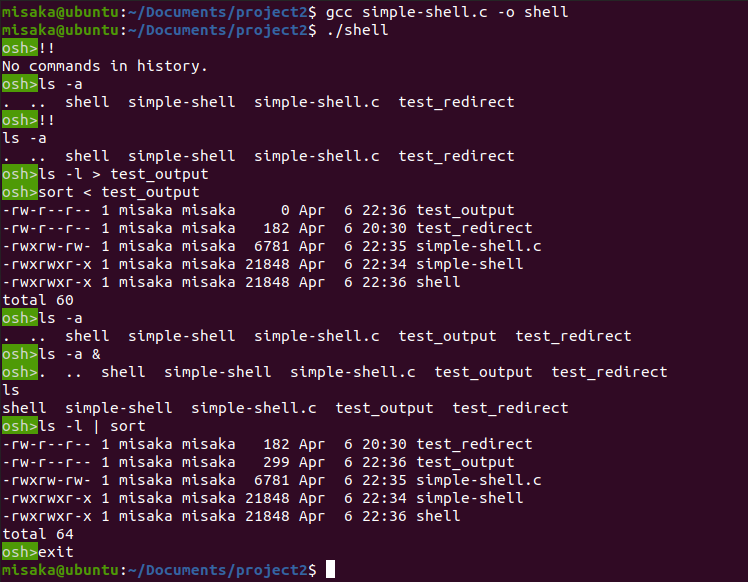
\includegraphics[width=400pt]{shell.png}
    \caption{Shell}
    \label{3}
\end{figure}



\section{Linux Kernel Module for Task Information}
In this project, we are required to write a Linux kernel module that use the /proc file system for displaying a task’s information based on its process identifier value pid.

\textbf{Design:} My key design is as follows:
\begin{itemize}
    \item In \textbf{proc\_write()}, i use \textbf{sscanf()} function to get the pid value from input.
    
    \item Memory allocation is different in the kernel. I use \textbf{kmalloc()} and \textbf{kfree()} to allocate memory.
    
    \item In \textbf{proc\_read()}, i use \textbf{pid\_task(find\_vpid(...), ...)} function to read the PCB information with a pid number.
    
    \item When there is a error (not valid pid number), i will print the kernel information to inform the user.
\end{itemize}

The code of pid.c is shown as follows.
\begin{lstlisting}[language = c]
#include <linux/init.h>
#include <linux/slab.h>
#include <linux/sched.h>
#include <linux/module.h>
#include <linux/kernel.h>
#include <linux/proc_fs.h>
#include <linux/vmalloc.h>
#include <asm/uaccess.h>

#define BUFFER_SIZE 128
#define PROC_NAME "pid"

/* the current pid */
static long l_pid;

static ssize_t proc_read(struct file *file, char *buf, size_t count, loff_t *pos);
static ssize_t proc_write(struct file *file, const char __user *usr_buf, size_t count, loff_t *pos);

static struct proc_ops proc_op = {
        .proc_read = proc_read,
        .proc_write = proc_write
};

static int proc_init(void)
{
        proc_create(PROC_NAME, 0666, NULL, &proc_op);
        printk(KERN_INFO "/proc/%s created\n", PROC_NAME);
	return 0;
}

static void proc_exit(void) 
{
        remove_proc_entry(PROC_NAME, NULL);
        printk( KERN_INFO "/proc/%s removed\n", PROC_NAME);
}

/**
 * This function is called each time the /proc/pid is read.
 * 
 * This function is called repeatedly until it returns 0, so
 * there must be logic that ensures it ultimately returns 0
 * once it has collected the data that is to go into the 
 * corresponding /proc file.
 */
static ssize_t proc_read(struct file *file, char __user *usr_buf, size_t count, loff_t *pos)
{
        int rv = 0;
        char buffer[BUFFER_SIZE];
        static int completed = 0;
        struct task_struct *tsk = NULL;

        if (completed) {
                completed = 0;
                return 0;
        }

        tsk = pid_task(find_vpid(l_pid), PIDTYPE_PID);
        if (tsk == NULL) {
                printk(KERN_INFO "Not a valid pid %ld\n", l_pid);
                return 0;
        }
        completed = 1;
        rv = sprintf(buffer, "command = [%s] pid = [%ld] state = [%ld]\n", tsk -> comm, l_pid, tsk -> state);
        if (copy_to_user(usr_buf, buffer, rv)) {
                rv = -1;
        }

        return rv;
}

/**
 * This function is called each time we write to the /proc file system.
 */
static ssize_t proc_write(struct file *file, const char __user *usr_buf, size_t count, loff_t *pos)
{
        char *k_mem;

        k_mem = kmalloc(count, GFP_KERNEL);

        if (copy_from_user(k_mem, usr_buf, count)) {
		printk( KERN_INFO "Error copying from user\n");
                return -1;
        }

        sscanf(k_mem, "%ld", &l_pid);

        kfree(k_mem);

        return count;
}

/* Macros for registering module entry and exit points. */
module_init( proc_init );
module_exit( proc_exit );

MODULE_LICENSE("GPL");
MODULE_DESCRIPTION("Pid");
MODULE_AUTHOR("MisakaCenter");
\end{lstlisting}

The Makefile for this task is written as follows.
\begin{lstlisting}
obj-m := pid.o
all:
	make -C /usr/src/linux-5.11.3/ M=$(shell pwd) modules
clean:
	make -C /usr/src/linux-5.11.3/ M=$(shell pwd) clean
\end{lstlisting}

The result is shown as follows.
\begin{figure}[H]
    \centering
    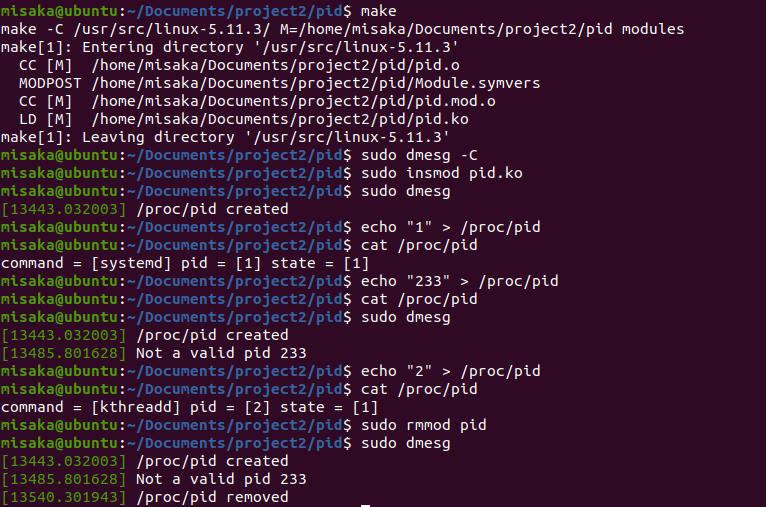
\includegraphics[width=400pt]{pid.png}
    \caption{Task information}
    \label{3}
\end{figure}

\end{document}